\documentclass{article}

\usepackage{fullpage}
\usepackage{parskip}
\usepackage{color}
\usepackage{listings}
\usepackage{amsmath}
\usepackage{graphicx}
\usepackage{caption}
\usepackage{subcaption}
\usepackage{wrapfig}

\lstset{basicstyle=\ttfamily}
\lstset{keywordstyle=\ttfamily\bfseries}
\lstset{language=LISP}
\lstset{columns=fullflexible}

\begin{document}
\title{Program Synthesis for DNA Strand Displacement}
\author{Kendall Stewart, Anthony Ha, Martin Kellogg}

\maketitle

\section{Introduction}

DNA computing seeks to leverage the chemical properties
of DNA molecules as a computational substrate.
From a medical perspective, DNA computing can enable the
construction of complex devices at a cellular scale for more precise
diagnostic tests or drug delivery. From a computer architecture perspective,
DNA is capable of performing massively parallel computations with very low
power consumption.

The feasibility of DNA computing was first demonstrated by encoding the
Hamiltonian Path Problem into DNA~\cite{adelman}. This encoding was constructed
by hand, but recent work has advanced DNA strand displacement reactions as a
primitive for DNA computation, because they can implement a wide
range of algorithms and devices, including boolean circuits~\cite{strands},
oscillators~\cite{dsd}, and neural networks~\cite{strandnn}.

Because of their boolean completeness, strand displacement reactions are
theoretically capable of implementing binary arithmetic operations. However,
some operations (such as multiplication) require a large number of
boolean gates, and strand-based boolean gates do not scale as well as
silicon-based gates; even moderately-sized systems begin to suffer noise
from unwanted interactions. Strand displacement reactions are capable
of more than just boolean
logic, so an arithmetic operation can be implemented with a set of
fewer, more complex strand displacement gates. However, reasoning about the
behavior of complex reactions is difficult for humans.

A formal semantics for strand displacement reactions is provided in the
description of DSD~\cite{dsd}, a programming language for specifying and
simulating DNA strand displacement circuits. Given a set of initial strand
species (reactants), DSD applies reduction rules to infer the intermediate and
final strand species (products), and creates a directed reaction graph with
edges between reactants and products, weighted by the rate of each reaction.
This graph, along with ordinary differential equations derived from the rates,
are used to simulate the strand displacement system.
Ignoring rates, the structure of the unweighted reaction graph encodes
conditions that are necessary (but not sufficient) for some product to have a
particular meaning. For instance, if all paths leading to a product include both
initial species $A$ and initial species $B$, the product could
represent $A \land B$.

\section{Overview of Our Approach}

We implemented an interpreter for the semantics of
DSD in Rosette~\cite{rosette}. By writing predicates
over the graph structure (in Rosette), we can ask
the solver to provide DNA structures that implement
interesting gates. For instance, we can ask the solver ``given
reactant $A$ and reactant $B$, find a system of gates where the
product represents $A \land B$". The solver is able to solve this
query and generate a gate that is semantically equivalent to
the best human design. We also synthesized an OR gate that
is simpler than the state-of-the-art human design while
retaining the semantics of OR.

The primary contributions of our work are:
\begin{enumerate}
\item
  An implementation in Rosette of both the detailed
  and infinite semantics for DSD, as an interpreter for
  strand displacement reactions.

\item
  An evaluation of this interpreter's usefulness for synthesizing
  implementations of simple boolean circuits as strand displacement
  reactions.

\item
  A novel OR gate that is specialized to two-input reactions and
  is dramatically smaller than existing human designs.
\end{enumerate}

\section{Algorithms and Encodings}

\subsection{Syntactic Encoding}

The core syntactic unit of DSD is a \emph{domain}, which identifies
a unique sequence of DNA bases.  Identifiers ending
in a \lstinline{^} represent short (or \emph{toehold}) domains,
while all other identifiers represent long domains.
Individual bases in the sequence are arbitrary, but distinct identifiers must
map to non-interfering sequences.
Every domain has a \emph{complement}, which is denoted
with a \lstinline{*} after the identifier. A domain's complement is
the Watson-Crick complement of the underlying bases: \lstinline{A} and \lstinline{T}
are complementary, and \lstinline{C} and \lstinline{G} are complementary.  
For example, if \lstinline{1^} is \lstinline{ACTG}, then \lstinline{1^*}
is \lstinline{TGAC}.

DNA in solution can be either single or double-stranded.
In double-stranded DNA, a sequence of bases is bound with its complement.
In DSD, a \emph{strand} is a single-stranded sequence of zero or more domains, for
example \verb;<1 2 3>; (which can also be written as the rotationally symmetric
\verb;{3 2 1};).
A \emph{gate} is a double-stranded sequence of one or more domains,
along with optional single-stranded overhangs on the top and bottom of each
side, for example \verb;<1>{2}[3 4]{5}<6>;.
Two gates may also share an upper or lower strand. If \verb;G1; and \verb;G2;
are gates, upper-strand sharing is written \verb;G1::G2; and lower-strand
sharing is written \verb;G1:G2;.

Our encoding of DSD's syntactic constructs is straightforward.
Long domains are encoded as integers, while
short domains are integers wrapped in a \verb;toehold; struct.
The complement operation is also a \verb;struct;.
Sequences of domains are encoded as lists, and strands are lists
tagged with the type (upper, lower, or double-stranded). Gates
are a five-tuple of their constituent strands.
Example syntactic encodings are shown in Table~\ref{table:encoding-example}.

\begin{table}
\begin{tabular}{|l|l|l|} \hline
Construct     & DSD Syntax    & Encoding                      \\ \hline
Long Domain   & \verb;0;      & \verb;0;                      \\ \hline
Toehold       & \verb;1^;     & \verb;(toehold 1);            \\ \hline
Complement    & \verb;1^*;    & \verb;(complement (toehold 1)); \\ \hline
Upper Strand  & \verb;<0 1^>; & \verb;(upper-strand (list 0 (toehold 1))); \\
\hline
Gate          & \verb;<1>{2^*}[3 4]{5}; &
\begin{lstlisting}
(gate
  (upper-strand (list 1))
  (lower-strand (list (complement (toehold 2))))
  (duplex-strand (list 3 4))
  (lower-strand (list 5))
  (upper-strand '()))
\end{lstlisting}
\\
\hline
\end{tabular}
\caption{Example of syntactic encoding.}
\label{table:encoding-example}
\end{table}

\subsection{Semantic Encoding}
\subsubsection{Reduction Rules}
DSD models the behavior of DNA strand displacement reactions with
\emph{reduction rules}---pattern-based rewrite rules
that model the conditions for and outcomes of a known reaction
involving DNA molecules. Reduction rules are also associated with
reaction rates, which model the kinetics of each chemical reaction.

The DSD specification refers to the set of reduction rules being used
as the level of \emph{semantic abstraction}, and defines four such levels.
More refined levels
use more rules, and produce more intermediate species. The
coarser abstractions use fewer rules (and merge some rules together) and
elide intermediate species.

Our encoding implements the coarsest semantic abstraction level,
the \emph{infinite} abstraction. This abstraction only has one
rule (rule RP) which describes binding interactions between a strand and a gate
that can lead to a strand displacement reaction (where a strand is
released from the gate). The infinite abstraction also allows for the strand
displacement reaction itself (rule RD)
to be merged into the RP reaction.
Rules RP and RD, and an outline of their merged encoding in Rosette, are shown in
Figure~\ref{figure:example-rule}. The outermost \verb;match*; expression
performs a purely syntactic match to check whether the species have
the correct type and bind their fields to variable names.
The inner \verb;match; and \verb;cond;
expressions discover if the domains of the input species satisfy
the requirements of the rule. If so, the result is a \verb;reaction;,
(a 4-tuple containing the input strand and gate, and the
output strand and gate). The empty list represents a reaction that
does not occur.

\begin{figure}[h]

\begin{subfigure}[c]{0.5\textwidth}
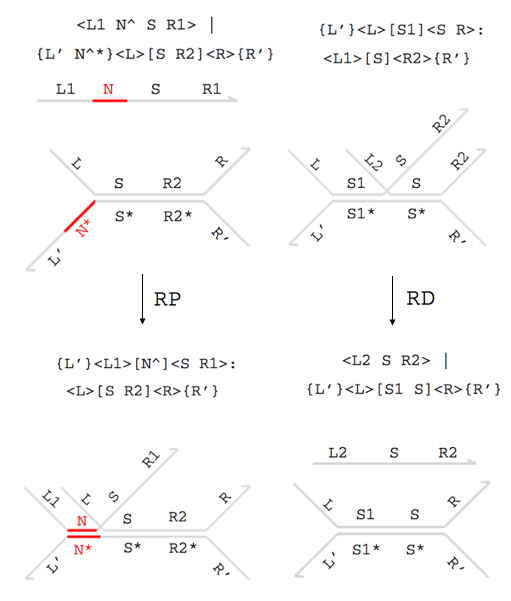
\includegraphics[width=\textwidth]{figures/rule-merge.png}
\end{subfigure}
~
\begin{subfigure}[c]{0.5\textwidth}
\begin{lstlisting}[basicstyle=\footnotesize\ttfamily]
(define (rule-rp strand-in gate-in)
  (match* (strand-in gate-in)
    [ ((upper-strand upper)

       (gate
        (upper-strand left-upper)
        (lower-strand left-lower)
        (duplex-strand duplex)
        (lower-strand right-lower)
        (upper-strand right-upper)))

      (match (toehold-search upper left-lower)
        ; no matching toehold, no reaction
        [ '() (reaction strand-in gate-in '() '()) ]

        ; matching toeholds
        [ (list ...)

          ; conditional merge with other rules
          (cond
            ...
            ; strand displacement
            [ ...
               (reaction
                strand-in gate-in
                (upper-strand ...)
                (gate ...)) ]) ]) ]

    [ (_ _) (reaction strand-in gate-in '() '()) ]))
\end{lstlisting}
\end{subfigure}
\caption{
DSD rules RP and RD, and their encoding as a merged rule, \lstinline{rule-rp} in
Rosette.  On the left, all identifiers (\lstinline{S}, \lstinline{R2}, etc.)
represent domain concatenations (lists of domains), except for \lstinline{N},
which represents a single toehold domain.
}
\label{figure:example-rule}
\end{figure}

\subsubsection{Reaction Graphs}

Given a set of input species, DSD computes a \emph{reaction graph} by applying
reduction rules to exhaustion (until no new species are produced). The vertices
of the graph are individual species, and edges between species indicate
reactions, weighted by the reaction rate. Reactions that require two species
join the edges from the two input species into a single edge leading to the
output. Reactions may also be reversible, indicated by a back edge from the
outputs to the inputs.

This graph
and its properties constitute the \emph{meaning} of a DSD program.
The reactions and their corresponding weights can be used to simulate
the progress of the system over time. At a coarser level of abstraction,
if we ignore rates, the structure of the graph can tell us whether or not
it is capable of carrying a particular meaning. The reaction
graph for a system representing an AND gate is shown in
Figure~\ref{figure:and-gate}. This system represents an AND gate
because all reactions that produce the strand \verb;<2 3>;
require (either directly or indirectly) both of the inputs.

We can write this requirement as a predicate in first-order logic, as
follows. Given a reaction graph $g$, and input strands $i_1$ and $i_2$:
\begin{equation}
\mathrm{isAndSystem}(g, i_1, i_2) =
\exists x \in \mathrm{strands}(g)\ .\ 
\forall p \in \mathrm{parents}_g(x)\ .\ 
\mathrm{requires}_g(p, i_1) \land \mathrm{requires}_g(p, i_2)
\label{eq:and-sys}
\end{equation}

Here, the function $\mathrm{strands}(g)$ returns the set of single strands in
the reaction graph $g$, and the function $\mathrm{parents}_g(x)$ returns
the set of parent reactions of the strand $x$ in graph $g$. The predicate 
$\mathrm{requires}_g(p,i)$ is true if the reaction $p$ cannot happen
(either directly or indirectly) without the strand $i$ in graph $g$.
It is easy to see that this predicate is satisfied for the graph in
Figure~\ref{figure:and-gate}.

\begin{figure}
\centering
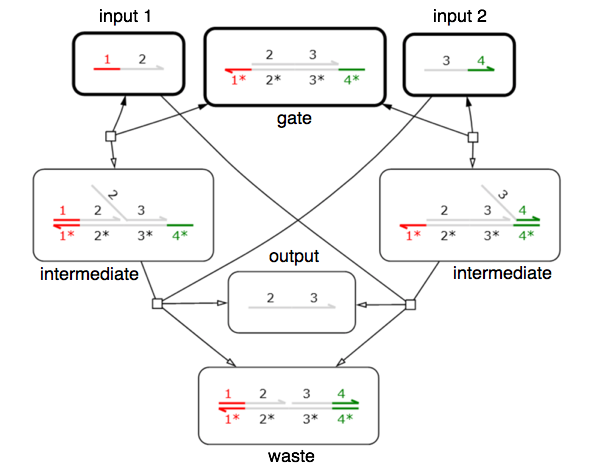
\includegraphics[width=0.5\textwidth]{figures/and-gate.png}
\caption{
The result of compiling the DSD program
\texttt{(<1\^{} 2>|<3 4\^{}>|\{1\^{}*\}[2 3]\{4\^{}*\})}
}
\label{figure:and-gate}
\end{figure}

\subsection{Solver-Aided Queries}
\subsubsection{"Synthesizing" DSD Programs}
Our goal is to apply a first-order predicate such as Equation~\ref{eq:and-sys}
to a reaction graph where the identity of one or more domains in the input
species is left symbolic, and then ask a solver to find bindings for the
symbolic variables such that the predicate is satisfied.

However, as specified by DSD, compiling a reaction graph requires applying
reduction rules until no new species are generated; this poses a problem
for symbolic execution, because the termination of this algorithm
depends on the identity of the species, and termination cannot be
predicated on symbolic values. Therefore, we finitize the computation
of the reaction graph by only considering a very small number of possible
reactions: the reactions between the initial species, and between
the products of those reactions and the initial species. The
resulting reaction graph will have a concrete size for a given
number of input strands and gates. Moreover, this finitization
is sufficiently powerful to reason about small systems such as the one
depicted in Figure~\ref{figure:and-gate}, where all relevant reactions
involve at least one of the input species and no relevant reaction
involves only intermediate products.

Since all reaction graphs are of a finite size and concrete shape,
writing a predicate such as the one in Equation~\ref{eq:and-sys} is
simple: sets are represented as lists, and we use Rosette's \verb;ormap; for
existential quantification and \verb;andmap; for universal quantification.
Applying this predicate to a reaction graph with symbolic inputs results
in a formula that can be passed to Rosette's \verb;solve; procedure.
Strictly speaking, this process is not inductive synthesis because it
does not require universal quantification over inputs -- we are simply
asking the solver to fill in a finite number of domain "holes" such that the
predicate is satisfied.

\subsubsection{Verified Continuous Integration}
As we were working on writing reduction rules, we were originally
checking our code with traditional \emph{ad hoc} testing. But,
since we were working in Rosette, we were able to use the \verb;verify;
form to check semantic properties of the rules and find bugs in the
form of counterexamples.  These verified tests were also used as regression
tests, and run by our CI server on each commit to help ensure that our code
stayed correct.

\section{Results}

\textcolor{red}{Description of AND and OR gate synthesis, limitations, etc}

\section{Teamwork}

To ensure that all three of us were involved in developing the encoding of
strand displacement reactions we used, much of the core infrastuctural code
that defines the encoding was developed by all three of us working on a single
screen. Once we had defined the core encoding, each team member worked on
making use of it in a particular way: Kendall, as the domain expert, worked
on implementing the rules and refining the encoding to perform better; Anthony
worked on building a implementing a normalization procedure (which required
some modifications to the encoding, as well) and a pretty printer/parser;
Martin created a test infrastructure (including a continuous integration server)
and then on writing verification procedures for the rules Kendall was
implementing (i.e. solver-aided exhaustive tests).

\section{Course Topics}

This project made heavy use of a solver-aided language: it is entirely dependent
on Rosette. In particular, we needed Rosette's ability to angelically execute
our symbolic programs (which represent reactions) and produce reactants that
cause the programs (reactions) to have the desired behavior---our synthesis
task. We also used bounded verification to test that our more complex
rules were correct. All topics we required were covered by the class.

\begin{thebibliography}{9}

\bibitem{adelman}
L. M. Adleman,
“Molecular computation of solutions to combinatorial problems,”
Science, vol. 266, no. 5187, pp. 1021–1024, Nov. 1994.

\bibitem{strands}
D. Y. Zhang and G. Seelig,
“Dynamic DNA nanotechnology using strand-displacement reactions,”
Nature Chemistry, vol. 3, no. 2, pp. 103–113, Feb. 2011.

\bibitem{dsd}
M. R. Lakin, S. Youssef, L. Cardelli, and A. Phillips,
“Abstractions for DNA circuit design,”
Journal of The Royal Society Interface, vol. 9, no. 68, Jul. 2011.

\bibitem{strandnn}
L. Qian, E. Winfree, and J. Bruck, “Neural network computation with DNA strand
displacement cascades,” Nature, vol. 475, no. 7356, pp. 368–372, Jul. 2011.

\bibitem{rosette}
  E. Torlak and R. Bodik, “A lightweight symbolic virtual machine for solver-aided host languages,” Programming Language Design and Implementation (PLDI), vol. 49, no. 6, pp. 530-541, 2014.

\end{thebibliography}

\end{document}
